\documentclass[10pt,twocolumn,letterpaper]{article}

\usepackage{cvpr}
\usepackage{times}
\usepackage{epsfig}
\usepackage{graphicx}
\usepackage{amsmath}
\usepackage{amssymb}
\usepackage{booktabs}
\usepackage{array}
\usepackage{enumitem}
\usepackage{tikz}
\usetikzlibrary{positioning, arrows.meta, shapes.geometric, calc, fit, backgrounds}
\usepackage[breaklinks=true,bookmarks=false]{hyperref}
\usepackage{microtype}
\usepackage{balance}

\cvprfinalcopy
\def\cvprPaperID{****}
\def\httilde{\mbox{\tt\raisebox{-.5ex}{\symbol{126}}}}
\setcounter{page}{1}

\begin{document}

%%%%%%%%% TITLE
\title{RGB-to-Velocity Imitation Learning for Quadrotor Navigation in FiGS}

\author{
\begin{tabular}{ccc}
Rahul Ayanampudi & Aditya Kothari & Yash Rampuria \\
AeroAstro Department & AeroAstro Department & AeroAstro Department \\
Stanford University & Stanford University & Stanford University \\
{\tt\small rayanam@stanford.edu} & {\tt\small kothari1@stanford.edu} & {\tt\small yashr@stanford.edu}
\end{tabular}
}

\maketitle

%%%%%%%%% ABSTRACT
\begin{abstract}
We present an end-to-end imitation-learning pipeline for goal-conditioned vision-based quadrotor navigation in the FiGS Gaussian-Splatting simulator. A privileged Model Predictive Controller (MPC) flies a quadrotor along Rapidly-exploring Random Tree (RRT)-planned, minimum-snap reference trajectories through reconstructed 3D scenes, producing synchronized RGB video and state logs. From these rollouts we train a compact student policy that maps a $T{=}4$-frame RGB history, monocular depth from a frozen Depth Anything V2 Small (DA2-S) branch, and a low-dimensional goal vector to a receding-horizon sequence of $H{=}10$ velocity commands $[v_x, v_y, v_z, \dot{\psi}]$. The visual backbone is ImageNet-pretrained ResNet-18 fused with DA2 depth features via LayerNorm cross-attention, followed by a single-layer GRU and a goal-conditioned MLP head. Training uses flightroom-only expert data; held-out flightroom validation trajectories and cross-scene backroom rollouts support offline and closed-loop validation; packardpark is reserved for zero-shot OOD test. After behavior cloning, we run two rounds of DAgger with an MPC re-solve oracle and fine-tune with balanced 50/50 sampling between expert and policy-visited windows. We then fine-tune the resulting checkpoint with on-policy PPO in full-length FiGS rollouts, using dense progress and settling-aware rewards.
\end{abstract}

%%%%%%%%% BODY TEXT
\section{Introduction}
\label{sec:intro}

Autonomous quadrotor navigation in cluttered environments requires fast perception, short-horizon decision-making, and stable tracking of dynamically feasible commands. Classical robotics stacks decompose this into perception, mapping, planning, and control. The decomposition is interpretable but accumulates latency when the vehicle moves quickly through visually complex scenes. Recent systems instead learn compact visuomotor policies that map onboard observations to local trajectories or commands, retaining only a thin low-level controller for stabilization~\cite{loquercio2021learning,low2024sousvide}.

This paper describes the implementation of an RGB-and-depth-to-command quadrotor policy for the FiGS simulator. FiGS couples physics-accurate ACADOS dynamics with a 3D Gaussian-Splatting (3DGS) renderer that produces RGB, depth, and CLIP-semantic views of reconstructed real-world scenes~\cite{low2024sousvide,kerbl2023gaussian}. A privileged MPC, given the planned reference trajectory, generates expert rollouts. The student policy sees the most recent four RGB frames, monocular depth from a frozen Depth Anything V2 Small (DA2-S) branch, and a goal vector, and must reproduce the expert's intent through a velocity-command interface.

The key engineering choices are (i) to predict a short \emph{command horizon} rather than a single instantaneous command, and (ii) to condition the policy on an explicit \emph{goal vector} (unit heading plus scale-normalized distance) alongside RGB. At each policy step the network outputs ten future commands of the form
\begin{equation}
\label{eq:command}
\mathbf{u}_t = \begin{bmatrix} v_x & v_y & v_z & \dot{\psi} \end{bmatrix}^\top \in \mathbb{R}^4,
\end{equation}
where $v_x, v_y, v_z$ are commanded world-frame linear velocities and $\dot{\psi}$ is the commanded yaw rate. Only the first command is executed before re-planning from the newest camera frames; the remaining nine are training-time supervision that shape the learned representation. A cascaded P-controller already present in FiGS consumes this four-vector and produces the low-level thrust and body-rate inputs $[u_f, \omega_x, \omega_y, \omega_z]$ to the ACADOS integrator, so the learned policy never has to model attitude or thrust dynamics directly.

Goal-vector conditioning addresses a fundamental limitation of purely RGB-based mapless navigation: an image sequence does not directly encode where the drone should \emph{go} or \emph{how far} it still has to travel. By supplying a unit heading toward the trajectory goal and a scale-normalized scalar distance to that goal, the policy receives a globally consistent reference direction \emph{and} a monotonic proximity signal. Both are cheap to compute, require no map, and provide meaningful learning signals that distinguish ``fly toward the goal while avoiding obstacles'' from ``follow a visually similar path in the wrong direction'' and ``slow down because the goal is near'' from ``cruise.''

Our contribution is fourfold: (i) a data-generation pipeline that turns recorded MPC rollouts in FiGS into goal-conditioned supervised $([\mathcal{I}_t,\mathbf{g}_t], \mathbf{U}^{*}_{t:t+H-1})$ training pairs, where $\mathbf{g}_t$ is the per-step goal vector (unit heading concatenated with scale-normalized distance); (ii) a ResNet-18--DA2-S--cross-attention--GRU--\emph{goal-conditioned}~MLP architecture; (iii) a training procedure that combines behavior cloning with two rounds of MPC-oracle DAgger and balanced expert/policy sampling to produce the deployment checkpoint; and (iv) an evaluation and RL fine-tuning protocol with offline metrics, closed-loop FiGS rollouts on flightroom val and backroom, zero-shot packardpark test, and optional PPO post-training on full expert trajectories.

\section{Related Work}
\label{sec:related}

Learning-based quadrotor navigation has moved increasingly toward direct prediction of local trajectories or commands from onboard observations. Loquercio \etal~\cite{loquercio2021learning} showed that high-speed flight through cluttered environments can be learned by mapping noisy sensory observations to collision-free receding-horizon trajectories.

SOUS VIDE is the closest system-level precedent for our project. Low \etal~\cite{low2024sousvide} introduced FiGS and used a privileged expert MPC to collect large image/action datasets, training their SV-Net policy on color, optical flow, and IMU streams to produce low-level body-rate and thrust commands. We borrow FiGS and the expert-distillation philosophy but intentionally simplify the student interface: RGB and frozen monocular depth at deploy time, and velocity-level rather than body-rate output, by sitting the policy on top of an in-tree velocity controller that SOUS VIDE did not use as the student's deployment interface. This isolates the visual representation-learning component and makes failures easier to attribute.

Bhattacharya \etal~\cite{bhattacharya2024vision} compare convolutional, recurrent, and vision-transformer policies for end-to-end quadrotor obstacle avoidance. Their results motivate future transformer comparisons; we use ResNet-18 + GRU here as a strong, compact baseline that fits within our simulator-iteration budget.

\subsection{Privileged imitation and dataset aggregation}

Our training procedure follows privileged imitation: an expert with access to information unavailable at deployment supervises a sensorimotor policy that sees only deployable observations, in the spirit of Learning by Cheating~\cite{chen2020learning}. Pure behavior cloning is not sufficient for sequential control because the learned policy induces its own state distribution and compounds small errors. DAgger~\cite{ross2011reduction} iteratively rolls out the learned policy, queries the expert on the states the policy actually visits, and aggregates those labels into the training set. We use a \emph{proper} DAgger oracle: at each policy-visited state, the FiGS VehicleRateMPC is re-solved from the current state and the planned next-step velocity and yaw rate become the label. Each DAgger round collects extended-horizon rollouts on flightroom training trajectories only; backroom and packardpark remain held out. After round~$2$, we fine-tune with \emph{balanced} batch sampling that mixes round-$0$ expert windows and round-${\geq}1$ policy-visited windows in equal proportion, yielding the \texttt{dagger\_balanced\_r12} deployment checkpoint used for closed-loop evaluation and RL warm-start.

\subsection{Visual and temporal representations}

The visual backbone is ResNet-18~\cite{he2016deep}, initialized with ImageNet weights and used as a per-frame feature extractor. Since a single image cannot infer approach speed or ego-motion reliably, we process the resulting feature sequence with a GRU~\cite{cho2014learning}. Depth-foundation models such as Depth Anything V2~\cite{yang2024depthanythingv2} supply geometry-aware features without changing the velocity-command interface. We use the Small (ViT-S) variant, frozen at train and deploy time, fused with ResNet-18 RGB features through LayerNorm cross-attention before the GRU. Relightable 3DGS photometric domain randomization is deferred; we instead apply color jitter, blur, brightness/gamma, and injected frame latency during BC and DAgger training.

\section{Problem Formulation}
\label{sec:formulation}

The simulator evolves in discrete control steps indexed by $t$ at $20\,\mathrm{Hz}$. At each step the onboard camera returns an RGB image $I_t \in \mathbb{R}^{H_I \times W_I \times 3}$. A rolling buffer stores the most recent $T$ frames,
\begin{equation}
\label{eq:obs}
\mathcal{I}_t = (I_{t-T+1}, I_{t-T+2}, \ldots, I_t),
\end{equation}
and the goal vector concatenates a unit heading in the world horizontal plane pointing from the drone's current XY position $\mathbf{p}_t$ to the trajectory end-point $\mathbf{p}_{\mathrm{goal}}$ with a scale-normalized scalar distance to that endpoint:
\begin{equation}
\label{eq:goalheading}
\mathbf{h}_t = \frac{[\mathbf{p}_{\mathrm{goal}} - \mathbf{p}_t]_{xy}}
                    {\|[\mathbf{p}_{\mathrm{goal}} - \mathbf{p}_t]_{xy}\|_2} \in \mathbb{R}^2,
\qquad
\tilde{d}_t = \frac{\|[\mathbf{p}_{\mathrm{goal}} - \mathbf{p}_t]_{xy}\|_2}{d_{\mathrm{scale}}} \in \mathbb{R}_{\geq 0},
\qquad
\mathbf{g}_t = (\mathbf{h}_t,\; \tilde{d}_t) \in \mathbb{R}^3.
\end{equation}
The characteristic scale $d_{\mathrm{scale}}{=}5\,\mathrm{m}$ keeps $\tilde{d}_t$ within roughly $[0, 1]$ for our sub-trajectory lengths; it is a fixed hyperparameter rather than a learned statistic so it stays stable across DAgger rounds and new scenes. The unit heading tells the policy \emph{which way} to go, and the normalized distance tells it \emph{how far}, giving it a direct deceleration signal as it approaches the endpoint.

Together $(\mathcal{I}_t, \mathbf{g}_t)$ form the full observation available to the learned policy at test time. The finalized implementation uses $T{=}4$, image resolution $224\times224$.

The policy predicts a horizon of $H{=}10$ four-dimensional commands:
\begin{equation}
\label{eq:horizon}
\hat{\mathbf{U}}_{t:t+H-1} = (\hat{\mathbf{u}}_t, \ldots, \hat{\mathbf{u}}_{t+H-1}) \in \mathbb{R}^{10 \times 4}.
\end{equation}
At $20\,\mathrm{Hz}$ the horizon spans $0.5\,\mathrm{s}$ of future commands. The runtime wrapper executes only $\hat{\mathbf{u}}_t$ before re-planning from the next observation:
\begin{equation}
\label{eq:policy}
\pi_\theta : \bigl(\mathbb{R}^{4 \times 3 \times 224 \times 224},\; \mathbb{R}^3\bigr) \rightarrow \mathbb{R}^{10 \times 4}.
\end{equation}

The expert supervises $\pi_\theta$ via horizons $\mathbf{U}^{*}_{t:t+H-1}$ derived from recorded MPC rollouts. The expert is allowed privileged simulator state during label generation; the student sees only $(\mathcal{I}_t, \mathbf{g}_t)$ at inference. The goal vector $\mathbf{g}_t$ is computable from the drone's state and the mission objective, both of which are available without a map.

\section{System Overview}
\label{sec:overview}

Figure~\ref{fig:system} summarizes the training and deployment paths. Training begins with closed-loop expert rollouts in FiGS, each driven by a privileged body-rate MPC tracking an RRT$^{*}$/min-snap reference trajectory through a 3DGS scene. For each rollout the simulator emits synchronized RGB, depth, and semantic video and a complete state and control log. From these we extract $(\mathcal{I}_t, \mathbf{U}^{*}_{t:t+H-1})$ samples and train the ResNet--DA2 policy by behavior cloning. DAgger then rolls the trained policy in FiGS on flightroom training trajectories, relabels each policy-visited state with the MPC re-solve oracle, and appends those windows to the dataset before balanced fine-tuning.

\begin{figure*}[t]
\centering
\resizebox{0.98\textwidth}{!}{%
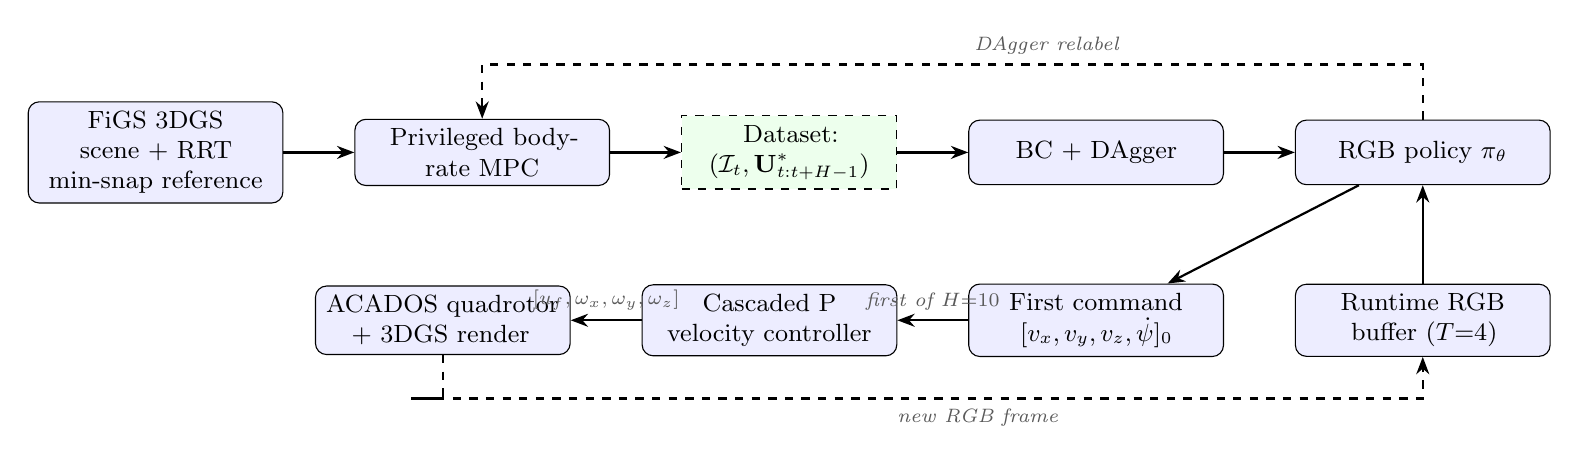
\begin{tikzpicture}[
    node distance=0.75cm and 0.9cm,
    block/.style={rectangle, draw, rounded corners, fill=blue!7,
                  minimum height=0.82cm, minimum width=2.2cm,
                  text width=2.2cm, align=center, font=\small},
    wide/.style={rectangle, draw, rounded corners, fill=blue!7,
                  minimum height=0.82cm, minimum width=3.0cm,
                  text width=3.0cm, align=center, font=\small},
    data/.style={rectangle, draw, dashed, fill=green!7,
                  minimum height=0.8cm, minimum width=2.5cm,
                  text width=2.5cm, align=center, font=\small},
    arr/.style={-{Stealth[length=2.2mm]}, thick},
    note/.style={font=\scriptsize\itshape, text=black!65}
]
\node[wide] (figs) {FiGS 3DGS scene + RRT min-snap reference};
\node[wide, right=of figs] (expert) {Privileged body-rate MPC};
\node[data, right=of expert] (dataset) {Dataset: $(\mathcal{I}_t, \mathbf{U}^{*}_{t:t+H-1})$};
\node[wide, right=of dataset] (train) {BC + DAgger};
\node[wide, right=of train] (policy) {RGB policy $\pi_\theta$};

\node[wide, below=1.25cm of policy] (runtime) {Runtime RGB buffer ($T{=}4$)};
\node[wide, left=of runtime] (cmd) {First command $[v_x,v_y,v_z,\dot{\psi}]_0$};
\node[wide, left=of cmd] (ctrl) {Cascaded P velocity controller};
\node[wide, left=of ctrl] (drone) {ACADOS quadrotor + 3DGS render};

\draw[arr] (figs) -- (expert);
\draw[arr] (expert) -- (dataset);
\draw[arr] (dataset) -- (train);
\draw[arr] (train) -- (policy);
\draw[arr] (runtime) -- (policy);
\draw[arr] (policy) -- (cmd);
\draw[arr] (cmd) -- node[note, above] {first of $H{=}10$} (ctrl);
\draw[arr] (ctrl) -- node[note, above] {$[u_f, \omega_x, \omega_y, \omega_z]$} (drone);
\draw[arr, dashed] (drone.south) |- ++(-0.4,-0.55) -| (runtime.south) node[note, pos=0.28, below] {new RGB frame};
\draw[arr, dashed] (policy.north) |- ++(0,0.7) -| (expert.north) node[note, pos=0.2, above] {DAgger relabel};
\end{tikzpicture}%
}
\caption{Training and deployment pipeline. The expert MPC generates rollouts that supply $(\mathcal{I}_t, \mathbf{g}_t, \mathbf{U}^{*}_{t:t+H-1})$ tuples (RGB history, goal vector, expert commands), where $\mathbf{g}_t$ is the unit heading toward the trajectory end-point concatenated with the scale-normalized scalar distance to that end-point. At deployment the policy reads a $T{=}4$ RGB and depth buffer \emph{and} the current goal vector, emitting a $10{\times}4$ command horizon; only the first command is forwarded to the in-tree velocity controller, which produces the low-level inputs consumed by the ACADOS integrator. DAgger relabels policy-visited states with the MPC re-solve oracle, preserving goal-vector labels computed from policy-visited positions.}
\label{fig:system}
\end{figure*}

\section{Model Architecture}
\label{sec:architecture}

The primary policy is a ResNet-18 + DA2-S + cross-attention--GRU--MLP network conditioned on a three-dimensional goal vector (heading + scale-normalized distance). An RGB-only ResNet baseline (ablation A0) omits the depth branch. The stem and first residual block of the ResNet are frozen to retain low-level ImageNet features. Figure~\ref{fig:arch} shows the RGB-only data flow; the production model inserts a frozen DA2-S depth map per frame, encodes it with a lightweight CNN to $256$-D, applies LayerNorm on both branches, and fuses via multi-head cross-attention (query = RGB, key/value = depth) with a second LayerNorm before the GRU.

\begin{figure}[t]
\centering
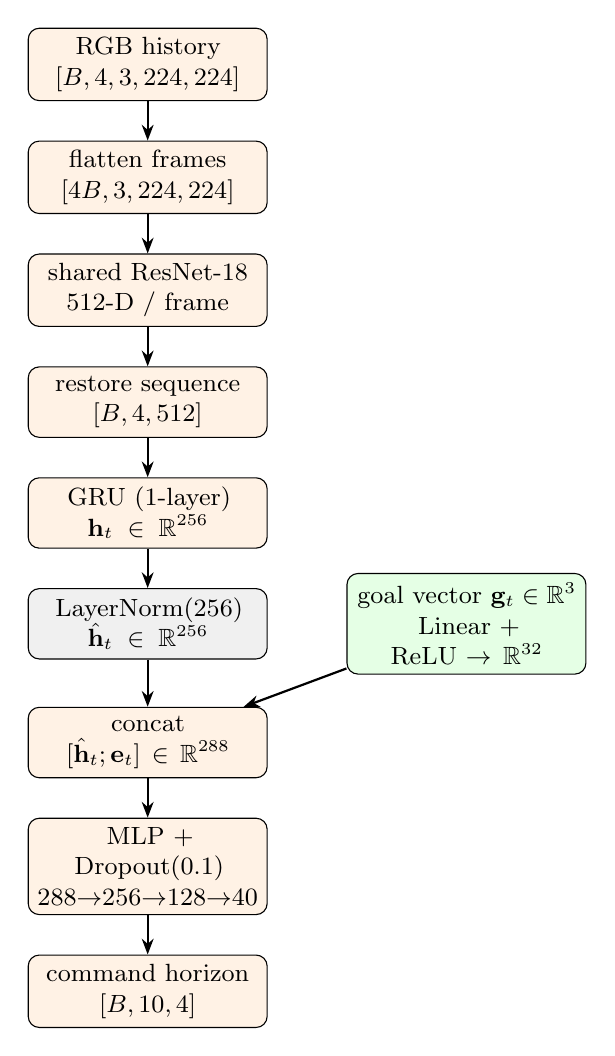
\begin{tikzpicture}[
    node distance=0.50cm,
    block/.style={rectangle, draw, rounded corners, fill=orange!10,
                  minimum height=0.72cm, minimum width=2.8cm,
                  text width=2.8cm, align=center, font=\small},
    gblock/.style={rectangle, draw, rounded corners, fill=green!10,
                  minimum height=0.72cm, minimum width=2.8cm,
                  text width=2.8cm, align=center, font=\small},
    rblock/.style={rectangle, draw, rounded corners, fill=gray!12,
                  minimum height=0.72cm, minimum width=2.8cm,
                  text width=2.8cm, align=center, font=\small},
    arr/.style={-{Stealth[length=2mm]}, thick},
]
\node[block] (input) {RGB history\\$[B,4,3,224,224]$};
\node[block, below=of input] (reshape) {flatten frames\\$[4B,3,224,224]$};
\node[block, below=of reshape] (resnet) {shared ResNet-18\\$512$-D / frame};
\node[block, below=of resnet] (seq) {restore sequence\\$[B,4,512]$};
\node[block, below=of seq] (gru) {GRU (1-layer)\\$\mathbf{h}_t \in \mathbb{R}^{256}$};
\node[rblock, below=of gru] (ln) {LayerNorm($256$)\\$\hat{\mathbf{h}}_t \in \mathbb{R}^{256}$};
\node[gblock, right=1.0cm of ln] (goal) {goal vector $\mathbf{g}_t \in \mathbb{R}^3$\\Linear + ReLU $\to \mathbb{R}^{32}$};
\node[block, below=0.6cm of ln] (cat) {concat $[\hat{\mathbf{h}}_t;\mathbf{e}_t] \in \mathbb{R}^{288}$};
\node[block, below=of cat] (mlp) {MLP + Dropout($0.1$)\\$288{\to}256{\to}128{\to}40$};
\node[block, below=of mlp] (out) {command horizon\\$[B,10,4]$};
\draw[arr] (input) -- (reshape);
\draw[arr] (reshape) -- (resnet);
\draw[arr] (resnet) -- (seq);
\draw[arr] (seq) -- (gru);
\draw[arr] (gru) -- (ln);
\draw[arr] (goal) -- (cat);
\draw[arr] (ln) -- (cat);
\draw[arr] (cat) -- (mlp);
\draw[arr] (mlp) -- (out);
\end{tikzpicture}
\caption{Goal-conditioned ResNet-18--GRU--MLP policy with regularization. LayerNorm on the GRU output normalizes the visual context to unit scale before concatenation with the goal embedding, ensuring both streams contribute proportionally. Dropout ($p{=}0.1$) is applied after each hidden ReLU in the MLP head.}
\label{fig:arch}
\end{figure}

\subsection{Visual encoder}

Each RGB frame is resized to $224\times224$ and normalized with ImageNet channel statistics
\begin{equation}
\label{eq:norm}
\mu = [0.485, 0.456, 0.406],\quad \sigma = [0.229, 0.224, 0.225].
\end{equation}
We use a torchvision ResNet-18 with the classification layer replaced by an identity, leaving the global-average-pooled $512$-D feature vector. A batch of shape $[B,4,3,224,224]$ is reshaped to $[4B,3,224,224]$, encoded in one forward pass, and reshaped back to
\begin{equation}
\label{eq:features}
\mathbf{Z} = (\mathbf{z}_{t-3}, \ldots, \mathbf{z}_t) \in \mathbb{R}^{B\times 4 \times 512}.
\end{equation}

\subsection{Temporal module and LayerNorm}

A single-layer GRU with hidden size $256$ consumes $\mathbf{Z}$ in chronological order; the final hidden state $\mathbf{h}_t \in \mathbb{R}^{256}$ summarizes the recent visual history. Before concatenation with the goal embedding, $\mathbf{h}_t$ is passed through a LayerNorm:
\begin{equation}
\hat{\mathbf{h}}_t = \mathrm{LayerNorm}(\mathbf{h}_t) \in \mathbb{R}^{256}.
\end{equation}
This is necessary because GRU hidden states can have varying magnitude, while the goal embedding is naturally bounded (it derives from a unit-vector input through a Linear + ReLU). Without normalization the 256-D visual stream would dominate the 32-D goal stream by sheer scale, effectively nullifying the goal-conditioning signal. LayerNorm brings both streams to a comparable scale so neither drowns the other.

\subsection{Goal-heading embedding and command head}

The three-dimensional goal vector $\mathbf{g}_t = (\mathbf{h}_t, \tilde{d}_t) \in \mathbb{R}^3$ (Eq.~\ref{eq:goalheading}) is passed through a single linear layer followed by ReLU to produce $\mathbf{e}_t \in \mathbb{R}^{32}$. The normalized GRU context and the goal embedding are concatenated:
\begin{equation}
\label{eq:concat}
\tilde{\mathbf{h}}_t = [\hat{\mathbf{h}}_t;\, \mathbf{e}_t] \in \mathbb{R}^{288}.
\end{equation}
A two-hidden-layer MLP ($288 \rightarrow 256 \rightarrow 128 \rightarrow 40$) predicts the flattened horizon, reshaped to $[B,10,4]$. ReLU activations are used between linear layers; Dropout ($p{=}0.1$) follows each hidden ReLU during training. Dropout is disabled at inference so predictions are deterministic. The goal-vector embedding is intentionally small (32-D) so the visual stream continues to carry primary information about obstacle layout; the heading supplies directional intent and the distance scalar supplies an approach-speed signal, neither overshadowing local geometry.

The network outputs commands in \emph{z-scored} space; the runtime wrapper de-standardizes them with the per-component statistics stored in the checkpoint.

\begin{table}[t]
\centering
\caption{Finalized model and interface settings.}
\label{tab:params}
\small
\begin{tabular}{@{}ll@{}}
\toprule
\textbf{Component} & \textbf{Setting} \\
\midrule
Input modality & RGB + DA2-S depth + goal vector \\
Frame history & $T=4$ frames \\
Image size & $224\times224$ \\
Depth branch & DA2-S (ViT-S), frozen; CNN encoder $\to 256$-D \\
Fusion & LayerNorm + cross-attention (RGB queries depth) \\
Goal heading & $[2]$ unit vector, world XY \\
Backbone & ResNet-18, ImageNet init.\ \\
Frozen layers & stem + first residual block \\
Frame feature size & $512$ \\
Temporal module & 1-layer GRU, hidden $256$ \\
Context normalization & LayerNorm($256$) on GRU output \\
Goal embedding & Linear($2{\to}32$) + ReLU \\
Concatenated context & $256 + 32 = 288$ \\
MLP head & $288\!\to\!256\!\to\!128\!\to\!40$ \\
MLP dropout & $p=0.1$ (hidden layers, train only) \\
Command horizon & $H=10$ steps \\
Command vector & $[v_x, v_y, v_z, \dot{\psi}]$ \\
Output tensor & $[B,10,4]$ \\
Inner controller & Cascaded P velocity controller \\
Inner-loop output & $[u_f, \omega_x, \omega_y, \omega_z]$ \\
Inference mode & Execute first command; re-plan \\
\bottomrule
\end{tabular}
\end{table}

\section{Dataset Generation in FiGS}
\label{sec:data}

We use closed-loop expert rollouts on flightroom for training; held-out flightroom validation trajectories (\texttt{071733}) and cross-scene backroom for offline/closed-loop validation; packardpark for zero-shot OOD closed-loop test only (never processed for BC or DAgger). Goal supervision uses the expert sub-trajectory endpoint $\mathbf{p}_{\mathrm{goal}} = \mathbf{X}_{\mathrm{ro}}[0{:}2,-1]$ everywhere (BC, val, DAgger, RL, and deploy). For each scene a planner produces RRT$^{*}$/min-snap reference trajectories, the expert MPC tracks each reference, and the simulator logs the synchronized RGB video, the full state trajectory, and the expert control history at $20\,\mathrm{Hz}$.

For every sub-trajectory we decode the corresponding RGB frames, resize them to $224\times224$, extract per-step linear velocity directly from the logged state, and compute world-frame yaw rate by finite-differencing the unwrapped yaw angle of the logged quaternion sequence:
\begin{equation}
\label{eq:psidot}
\dot{\psi}_k = (\mathrm{unwrap}(\psi(q_{k+1})) - \mathrm{unwrap}(\psi(q_k))) \cdot f_{\mathrm{ctl}},
\end{equation}
with $f_{\mathrm{ctl}} = 20\,\mathrm{Hz}$. In the same pass we compute the per-step goal vector (Eq.~\ref{eq:goalheading})---a unit heading from current XY to the trajectory end-point together with the scale-normalized scalar distance to that end-point. This yields a sequence of $(I_k, \mathbf{g}_k, [v_x, v_y, v_z, \dot{\psi}]_k)$ tuples per sub-trajectory.

A second pass enumerates training windows: for every length-$n$ sub-trajectory and every $k \in [T{-}1, n{-}H)$ we form a sample whose input is the four most recent frames ending at $k$ \emph{and} the goal vector at step $k$, and whose target is the next ten expert commands $[v_x, v_y, v_z, \dot{\psi}]_{k:k+H-1}$. Train/validation splits are assigned \emph{by sub-trajectory}, never by frame, to avoid the temporal leak that a frame-level random split would introduce. After the split, per-component means and standard deviations of the four command components are fit on the training set; the network is trained and evaluated entirely in z-scored space and de-normalized only at deployment. The goal distance is normalized by a fixed characteristic scale $d_{\mathrm{scale}}{=}5\,\mathrm{m}$ stored in the model config, so its scaling is constant across rounds without requiring dataset statistics.

Table~\ref{tab:dataset} summarizes the data split. Flightroom training runs (\texttt{064652}, \texttt{071718}, \texttt{071353}) supply BC and DAgger windows. The flightroom validation run (\texttt{071733}, 12 queries) and backroom are held out for offline and closed-loop validation. Packardpark is never included in processed training data; it is evaluated only via closed-loop rollouts.

\begin{table}[t]
\centering
\caption{Data split. Train = processed BC/DAgger; val = offline + in-domain closed-loop; test = OOD closed-loop only.}
\label{tab:dataset}
\small
\begin{tabular}{@{}lll@{}}
\toprule
\textbf{Split} & \textbf{Scenes / runs} & \textbf{Use} \\
\midrule
Train & flightroom (\texttt{064652}, \texttt{071718}, \texttt{071353}) & BC, DAgger, RL phase~1 \\
Val (in-domain) & flightroom \texttt{071733} & Offline + closed-loop \\
Val (cross-scene) & backroom & Offline + closed-loop \\
Test (OOD) & packardpark & Closed-loop only \\
\bottomrule
\end{tabular}
\end{table}

\section{Training Objective and DAgger}
\label{sec:training}

\subsection{Behavior cloning loss}

Let $\hat{\mathbf{U}}_{t:t+H-1}$ and $\mathbf{U}^{*}_{t:t+H-1}$ denote the predicted and expert horizons in z-scored space. The command loss is the mean squared error across the horizon:
\begin{equation}
\label{eq:mse}
\mathcal{L}_{\mathrm{cmd}} = \frac{1}{H \cdot 4} \sum_{i=0}^{H-1} \|\hat{\mathbf{u}}_{t+i} - \mathbf{u}^{*}_{t+i}\|_2^2.
\end{equation}
Because targets are z-scored using training-set statistics (Table~\ref{tab:stats}), all four command components contribute on roughly equal scales without an explicit per-component weight matrix.

A smoothness penalty discourages jittery horizons:
\begin{equation}
\label{eq:smooth}
\mathcal{L}_{\mathrm{smooth}} = \frac{1}{(H{-}1) \cdot 4} \sum_{i=0}^{H-2} \|\hat{\mathbf{u}}_{t+i+1} - \hat{\mathbf{u}}_{t+i}\|_2^2.
\end{equation}
The total loss is $\mathcal{L} = \mathcal{L}_{\mathrm{cmd}} + \lambda_s \mathcal{L}_{\mathrm{smooth}}$ with $\lambda_s = 0.05$.

\subsection{DAgger}

After BC convergence we run two DAgger rounds on flightroom training trajectories. The trained policy is rolled out in FiGS with extended horizons until goal, collision, or timeout; at every control step the MPC oracle re-solves from the policy's current state and supplies fresh velocity labels. Policy-visited windows are appended to the processed dataset and tagged by DAgger round. Per-component normalization statistics fit on round-$0$ data remain frozen across rounds. The final imitation checkpoint (\texttt{dagger\_balanced\_r12}) is obtained by fine-tuning with balanced sampling: each training epoch draws expert (round-$0$) and policy-visited (round~${\geq}1$) windows in a 50/50 ratio so recovery states are not drowned out by the original expert corpus.

\subsection{RL fine-tuning (PPO)}
\label{sec:rl}

After BC and two rounds of balanced DAgger produce a strong initializer (\texttt{dagger\_balanced\_r12/bc\_best.pt}), we fine-tune in FiGS with Proximal Policy Optimization (PPO)~\cite{schulman2017proximal}. The student remains a \emph{goal-conditioned velocity policy}: the same ResNet--DA2 fusion backbone, GRU context, and four-dimensional command head are warm-started from the imitation checkpoint; RL adds a diagonal Gaussian exploration head and a scalar value critic. Actions are sampled in z-scored command space and de-normalized before forwarding to the inner velocity controller.

\paragraph{Rollout protocol.} RL uses full expert validation trajectories (\texttt{071718} and \texttt{071353}, eight queries), not short training clips. Episodes start at the expert initial state (\texttt{expert\_x0}) with the goal at the trajectory terminal pose; rollouts run until goal settle, collision, or a 60\,s cap. A PID warmup phase stabilizes the drone before the learned policy takes control. Success requires both reaching the goal region and passing a settle detector (consecutive low-velocity steps). Depth at deploy time is computed live by frozen DA2-S (with configurable inference stride); collision checks use FiGS depth renders.

\paragraph{Rewards.} Dense step rewards combine progress toward the goal, heading alignment, a per-step living penalty, an action-smoothness penalty on consecutive commands, a bounding-box violation proxy, and a terminal bonus only when the settle detector fires. We do \emph{not} modify the FiGS renderer or use relightable 3DGS augmentation during RL.

\paragraph{Training schedule.} PPO collects one episode per iteration, batches four episodes before each policy update, and saves checkpoints every update. The simulator instance is reused across episodes on the same scene to amortize 3DGS load cost; transition RGB windows are stored in fp16 for memory efficiency. Held-out flightroom val (\texttt{071733}) and packardpark are reserved for post-training evaluation; a later phase introduces mixed mid-path starts for recovery training.

\paragraph{Checkpoints.} RL checkpoints store updated backbone weights plus RL head parameters (\texttt{log\_std}, critic). Episode-level CSV logs record success, settle status, and per-trajectory semantics for analysis alongside \texttt{latest} and \texttt{best} weight files.

\subsection{Regularization}

Three regularization mechanisms address the overfitting risk inherent in training on a small simulator dataset.

\paragraph{Per-frame color jitter.} At each training step, a fresh random photometric transform is independently applied to every frame in the $T$-frame input window before ImageNet normalization. The transform perturbs brightness ($\pm30\%$), contrast ($\pm30\%$), saturation ($\pm20\%$), and hue ($\pm5\%$). Applying independent transforms per frame is intentional: it prevents the model from using inter-frame color consistency as a proxy for ego-motion, forcing it to rely on structural rather than photometric features. No augmentation is applied to the validation set.

\paragraph{MLP dropout.} Dropout ($p{=}0.1$) is inserted after each hidden ReLU in the MLP prediction head. It is disabled at inference, so predictions are deterministic. Dropout is placed only in the head because the ResNet backbone is heavily pre-trained (and partially frozen) and the GRU is already regularized by weight decay.

\paragraph{LayerNorm + weight decay.} LayerNorm on the GRU output acts as implicit regularization by preventing the hidden state from growing unbounded. Combined with AdamW weight decay ($10^{-4}$), these mechanisms jointly constrain all three components.

\subsection{Training schedule}

We use AdamW with learning rate $3\!\times\!10^{-4}$, weight decay $10^{-4}$, mixed-precision training when CUDA is available, gradient clipping at norm $1.0$, batch size $16$, and a fixed seed of $0$ for 15 epochs. Each checkpoint carries the command-normalization statistics and image-preprocessing settings alongside the model weights; without them a checkpoint is not deployable, because the network outputs z-scored values that the runtime wrapper must de-normalize before forwarding to the inner controller.

\begin{table}[t]
\centering
\caption{Per-component command statistics fit on the flightroom training split. Units: m/s for $v_x,v_y,v_z$; rad/s for $\dot{\psi}$.}
\label{tab:stats}
\small
\begin{tabular}{@{}lrr@{}}
\toprule
Component & $\mu$ & $\sigma$ \\
\midrule
$v_x$        & $-0.0081$ & $0.4344$ \\
$v_y$        & $\phantom{-}0.0180$ & $0.5308$ \\
$v_z$        & $-0.0209$ & $0.1196$ \\
$\dot{\psi}$ & $\phantom{-}0.0216$ & $0.3514$ \\
\bottomrule
\end{tabular}
\end{table}

\section{Runtime Integration}
\label{sec:runtime}

Closed-loop deployment proceeds at the simulator's $20\,\mathrm{Hz}$ control rate. Each step reads the latest rendered RGB image, runs frozen DA2-S to produce a depth map (with optional inference stride), applies resize and ImageNet normalization, pushes RGB and depth into a four-frame rolling buffer, and computes the goal vector from the current drone position. Both modalities and the goal are forwarded to the policy; only the first of ten predicted commands is de-normalized and passed to the cascaded velocity controller.

\begin{table}[t]
\centering
\caption{Goal-conditioned receding-horizon policy step at every control update.}
\label{tab:runtime}
\small
\begin{tabular}{@{}p{0.95\linewidth}@{}}
\toprule
\textbf{Step} \\
\midrule
1. Read the latest RGB image from the simulator's renderer. \\
2. Run frozen DA2-S to produce a depth map (optional inference stride). \\
3. Resize RGB and depth to $224\times224$; apply ImageNet normalization to RGB (Eq.~\ref{eq:norm}). \\
4. Append RGB and depth to the four-frame rolling buffers. \\
5. Compute the goal vector $\mathbf{g}_t = (\mathbf{h}_t, \tilde{d}_t)$ from current XY position and stored goal (Eq.~\ref{eq:goalheading}). \\
6. Run the policy on RGB history, depth history, and $\mathbf{g}_t$. \\
7. Receive a $[1,10,4]$ command horizon. \\
8. Take the first command $[v_x, v_y, v_z, \dot{\psi}]_0$ and de-normalize it. \\
9. Forward it to the inner velocity controller, which produces $[u_f, \omega_x, \omega_y, \omega_z]$. \\
10. The simulator integrates the dynamics and renders the next image. \\
\bottomrule
\end{tabular}
\end{table}

The output interface is deliberately the velocity controller, not the body-rate MPC. Separating the visual-command generator from the inner stabilizer makes debugging easier: if the drone tracks a commanded velocity poorly, the issue lies with the inner controller's gains or with the integrator; if the predicted velocity is visually inappropriate (e.g.~commanding forward speed into a wall), the issue lies with the learned policy or the dataset.

\section{Experimental Setup}
\label{sec:experimental}

\textbf{Hardware.} All experiments run on a CUDA-11.8 / PyTorch-2.1 environment with mixed-precision training. The development machine uses an NVIDIA RTX 3050 Laptop GPU (4\,GB).

\textbf{Data.} Imitation training uses processed flightroom windows from expert runs \texttt{064652}, \texttt{071718}, and \texttt{071353}. Offline and closed-loop validation uses the held-out flightroom run \texttt{071733} (12 queries) and cross-scene backroom; packardpark is never processed for BC or DAgger and is reserved for zero-shot OOD closed-loop test only (Table~\ref{tab:dataset}).

\textbf{Expert characteristics.} The privileged MPC flies the quadrotor with an average linear speed of $0.75\,\mathrm{m/s}$ across the evaluation set, with peak speeds of $1.2$--$1.4\,\mathrm{m/s}$ during accelerations and decelerations. The mean expert flight duration is $6.67\,\mathrm{s}$ and the mean expert flight length is $5.18\,\mathrm{m}$. Individual rollouts range from short five-second indoor maneuvers ($\approx 3.1\,\mathrm{m}$) to longer ten-second outdoor flights ($\approx 8.9\,\mathrm{m}$). These numbers define the relevant scale for interpreting tracking and velocity errors: a $0.2\,\mathrm{m/s}$ velocity RMSE is roughly $25\%$ of the expert's average speed.

\textbf{Training schedule.} BC trains the \texttt{rgb\_da2\_crossattn\_v1} model (${\approx}10$ epochs) with photometric augmentations, LayerNorm, and MLP dropout on flightroom-only data. Two DAgger rounds follow on flightroom training trajectories with extended horizons and MPC re-labeling; the deployment checkpoint \texttt{dagger\_balanced\_r12/bc\_best.pt} is obtained by fine-tuning with balanced 50/50 sampling between round-$0$ expert windows and policy-visited recovery windows. RL fine-tuning (PPO, 100 episodes) warm-starts from that checkpoint on full \texttt{071718}/\texttt{071353} expert trajectories with expert-$x_0$ starts.

\section{Results}
\label{sec:results}

\subsection{Behavior-cloning training curves}

Figure~\ref{fig:curves} (left) plots behavior-cloning training and validation loss from an earlier RGB-only backroom $+$ packardpark baseline; the current flightroom \texttt{rgb\_da2\_crossattn} run uses the same z-scored command loss, smoothness penalty ($\lambda_\text{smooth}{=}0.05$), and regularization stack on the split in Table~\ref{tab:dataset}. In both settings the flat z-scored validation curve can mask continued improvement in physical-unit per-component error (right panel). Checkpoint selection uses \texttt{val\_mse\_overall} in physical units.

\begin{figure*}[t]
\centering
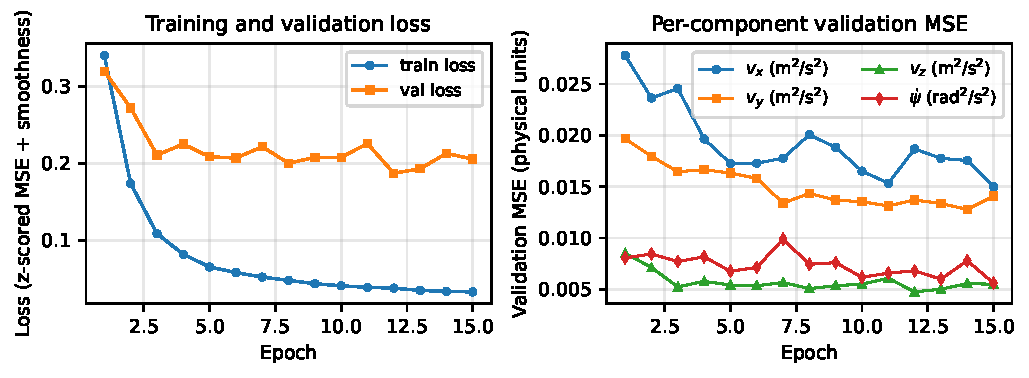
\includegraphics[width=0.95\textwidth]{figures/training_curves.pdf}
\caption{Behavior-cloning training curves from an earlier RGB-only backroom $+$ packardpark baseline (left: z-scored loss; right: physical-unit validation MSE). The current flightroom ResNet--DA2 run uses the same objective and regularization on the split in Table~\ref{tab:dataset}.}
\label{fig:curves}
\end{figure*}

\subsection{Offline validation: behavior cloning and balanced DAgger}

We evaluate checkpoints on the held-out flightroom (\texttt{071733}) and backroom validation splits. The primary deployment initializer is the balanced DAgger checkpoint (\texttt{dagger\_balanced\_r12/bc\_best.pt}), trained after two MPC-oracle DAgger rounds with 50/50 expert/policy window sampling. Table~\ref{tab:offline} reports offline metrics from an earlier RGB-only baseline; representative flightroom-val numbers for the DA2 BC checkpoint are linear-velocity RMSE $0.213\,\mathrm{m/s}$ and mean inference latency $10.4\,\mathrm{ms}$ on $21{,}006$ held-out windows. Balanced-DAgger offline and closed-loop numbers on the full val protocol are in progress.

\begin{table}[t]
\centering
\caption{Offline validation metrics in physical units (preliminary RGB-only baseline on an earlier backroom $+$ packardpark val split). The current pipeline evaluates \texttt{rgb\_da2\_crossattn} and \texttt{dagger\_balanced\_r12} on flightroom \texttt{071733} and backroom.}
\label{tab:offline}
\small
\begin{tabular}{@{}lrrrr@{}}
\toprule
 & \multicolumn{2}{c}{BC (round 0)} & \multicolumn{2}{c}{BC $+$ DAgger r2} \\
\cmidrule(lr){2-3}\cmidrule(lr){4-5}
Component                 & RMSE   & MAE   & RMSE   & MAE   \\
\midrule
$v_x$ (m/s)               & $0.131$ & $0.079$ & $0.122$ & $0.071$ \\
$v_y$ (m/s)               & $0.121$ & $0.072$ & $0.119$ & $0.067$ \\
$v_z$ (m/s)               & $0.075$ & $0.029$ & $0.074$ & $0.026$ \\
$\dot{\psi}$ (rad/s)      & $0.072$ & $0.044$ & $0.075$ & $0.041$ \\
\midrule
Linear velocity (norm)    & $0.112$ & --- & $0.107$ & --- \\
Latency, mean (ms)        & \multicolumn{2}{c}{$5.5$} & \multicolumn{2}{c}{$5.4$} \\
\bottomrule
\end{tabular}
\end{table}

\subsection{Horizon-step error}

Figure~\ref{fig:horizon} breaks down per-component RMSE across the ten predicted horizon steps for the preliminary RGB-only BC and DAgger checkpoints on an earlier val split. The current flightroom ResNet--DA2 model follows the same $H{=}10$ supervision; balanced-DAgger horizon curves on flightroom val are pending.

\begin{figure*}[t]
\centering
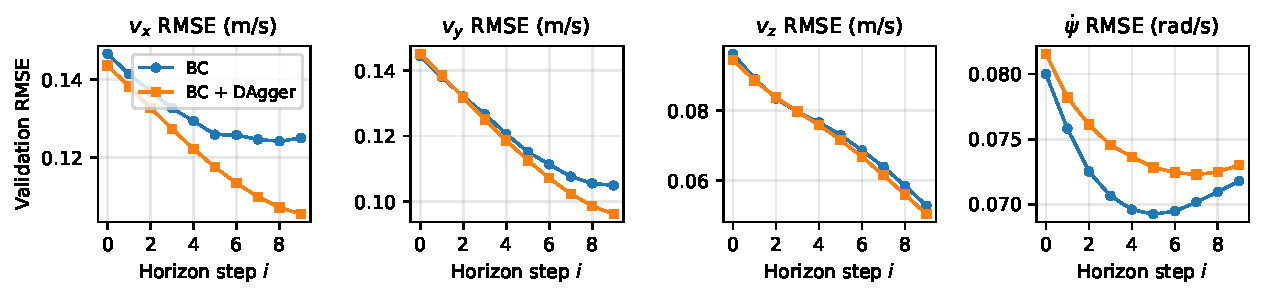
\includegraphics[width=0.95\textwidth]{figures/horizon_rmse.pdf}
\caption{Per-horizon-step RMSE for each command component on a preliminary RGB-only val split (BC round~$0$ vs.\ DAgger round~$2$).}
\label{fig:horizon}
\end{figure*}

\subsection{Closed-loop FiGS rollouts}
\label{sec:closedloop}

Closed-loop evaluation drives the trained policy through the velocity controller in a fresh simulator instance, starting from expert initial conditions and using the policy's own induced state distribution. We evaluate on three tiers: in-domain flightroom val (\texttt{071733}), cross-scene backroom, and zero-shot packardpark OOD test. A rollout is counted as a \emph{success} when the settle detector fires within the time cap (position/yaw tolerances plus consecutive low-velocity steps), not merely when the drone ends near the goal on timeout.

Table~\ref{tab:closedloop} reports preliminary closed-loop metrics from an early RGB-only BC checkpoint on backroom and packardpark; the current \texttt{rgb\_da2\_crossattn} + balanced DAgger checkpoint is evaluated on flightroom val, backroom, and packardpark with the same protocol. RL fine-tuning results (PPO on full expert trajectories) will be added once the 100-episode flightroom training run completes.

\begin{table}[t]
\centering
\caption{Preliminary closed-loop FiGS metrics (early RGB-only BC baseline). BR = backroom, PP = packardpark OOD test. Current pipeline evaluates \texttt{rgb\_da2\_crossattn} + balanced DAgger on flightroom val, backroom, and packardpark.}
\label{tab:closedloop}
\small
\begin{tabular}{@{}lcccc@{}}
\toprule
Metric & BR sub0 & BR sub2 & PP sub0 & Mean ($N{=}3$) \\
\midrule
Duration (s)                  & $5.0$   & $5.0$   & $10.0$  & $6.67$           \\
Steps                         & $100$   & $100$   & $200$   & ---              \\
Success                       & \checkmark & \checkmark & \checkmark & $100\,\%$ \\
BBox violations               & $0$     & $0$     & $0$     & $0\,\%$          \\
Pos.\ tracking RMSE (m)       & $0.246$ & $0.285$ & $0.284$ & $0.272\pm0.018$  \\
Final position error (m)      & $0.379$ & $0.248$ & $0.295$ & $0.308\pm0.054$  \\
Max position error (m)        & $0.384$ & $0.440$ & $0.497$ & $0.440\pm0.046$  \\
Vel.\ RMSE, norm (m/s)        & $0.161$ & $0.315$ & $0.176$ & $0.217\pm0.069$  \\
Yaw RMSE (rad)                & $0.034$ & $0.039$ & $0.051$ & $0.041\pm0.007$  \\
Path length, policy (m)       & $3.39$  & $3.81$  & $9.46$  & $5.55\pm2.77$    \\
Path length, expert (m)       & $3.06$  & $3.62$  & $8.86$  & $5.18\pm2.61$    \\
Model latency, mean (ms)      & $17.0$  & $13.2$  & $12.9$  & $14.4\pm1.9$     \\
Model latency, p95 (ms)       & $22.7$  & $16.3$  & $14.2$  & $17.7\pm3.6$     \\
Inner-loop latency, mean (ms) & $0.34$  & $0.45$  & $0.37$  & $0.39\pm0.05$    \\
\bottomrule
\end{tabular}
\end{table}

\begin{figure*}[t]
\centering
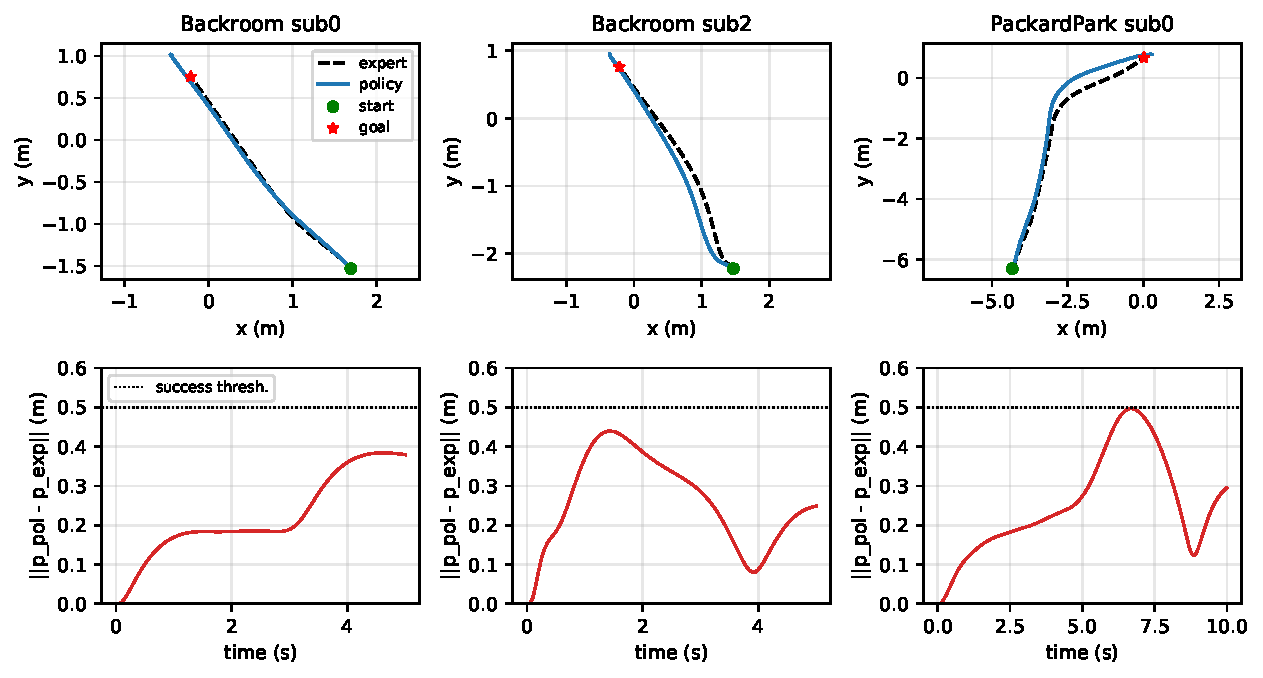
\includegraphics[width=0.95\textwidth]{figures/trajectory_overlay.pdf}
\caption{Closed-loop trajectory overlays (top row) and per-step position error (bottom row) for each rollout. The expert reference is dashed, the policy is solid, the start is green, and the goal is a red star. The dotted line in the bottom row marks the $0.5\,\mathrm{m}$ success threshold for final position error; all three rollouts finish below it.}
\label{fig:traj_overlay}
\end{figure*}

\subsection{Speed profile vs.\ the expert}

Figure~\ref{fig:speed} compares the speed magnitude $\lVert\mathbf{v}\rVert$ of the closed-loop policy and the recorded expert over time. The policy mirrors the expert's overall speed envelope but lags slightly during the deceleration phase of each rollout, ending with a small residual speed (visible as the non-zero tail at $t \to T$). This lag is responsible for the $\sim 7\%$ path over-shoot in Table~\ref{tab:closedloop} and is the most actionable failure mode: a tighter velocity controller (larger $K_v$) or a deceleration-aware training augmentation would likely close it.

\begin{figure*}[t]
\centering
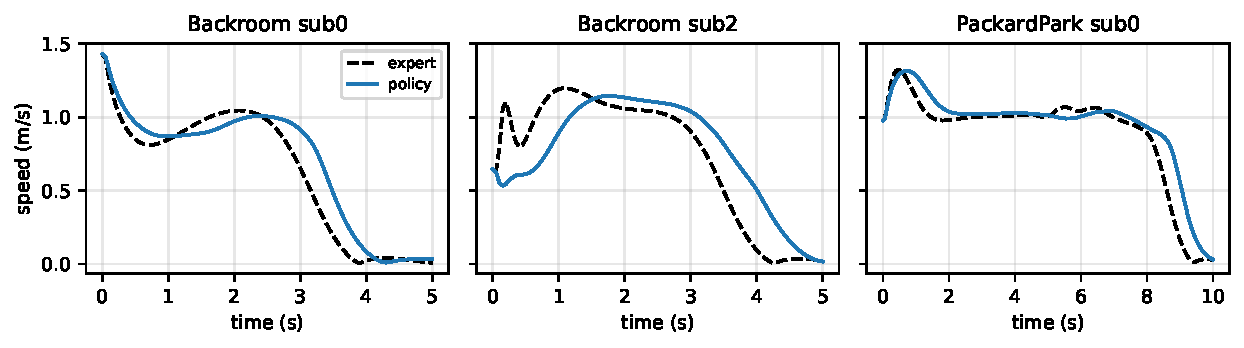
\includegraphics[width=0.95\textwidth]{figures/speed_profile.pdf}
\caption{Linear speed of the closed-loop policy (solid) vs.\ the recorded expert (dashed) for each rollout. The policy tracks the expert's speed envelope but lags during deceleration, producing the small path over-travel reported in Table~\ref{tab:closedloop}.}
\label{fig:speed}
\end{figure*}

\subsection{Qualitative rollout videos}

Each closed-loop rollout writes a $20\,\mathrm{Hz}$ first-person RGB video from the FiGS renderer (\emph{video.mp4} per rollout directory). These videos let a reader see the actual observation stream the policy received and confirm visually that the drone reaches the goal, traverses obstacles, and stays within the bounding box. The supplementary materials include the three videos from the runs in Table~\ref{tab:closedloop}.

\section{Ablations}
\label{sec:ablations}

We propose four ablations whose only purpose is to validate the implemented design choices; they are not alternative final systems. All ablation comparisons use the same scenes, seeds, and inner-controller gains.

\paragraph{Goal-vector conditioning.} Train an otherwise identical policy with the full goal vector zeroed (heading \emph{and} normalized distance both set to $\mathbf{0}$). Comparing this baseline to the full model on closed-loop success rate and position tracking RMSE isolates the contribution of the goal channel for mapless goal-seeking. We expect the goal-conditioned model to outperform the goal-free baseline most on longer or more meandering trajectories where visual context alone is ambiguous, and we expect the distance scalar specifically to reduce overshoot near the endpoint.

\paragraph{BC vs.\ balanced DAgger.} Compare the round-$0$ BC checkpoint against the \texttt{dagger\_balanced\_r12} checkpoint on closed-loop metrics (flightroom val, backroom, packardpark). Balanced sampling prevents policy-visited recovery windows from being swamped by the original expert corpus.

\paragraph{History length $T$.} Train identical architectures with $T \in \{1, 2, 4, 8\}$ (our default is $T{=}4$). Larger $T$ should improve $\dot{\psi}$ prediction the most, because yaw rate depends most strongly on inter-frame motion cues. $T{=}1$ is the no-temporal-context baseline.

\paragraph{Horizon length $H$.} Train with $H \in \{1, 5, 10, 20\}$. Larger $H$ acts as auxiliary supervision and should regularize the hidden state, but only the first step is executed. The expected shape is U-shaped: very short $H$ removes the regularization benefit; very large $H$ wastes capacity on increasingly noisy distant predictions.

\begin{table}[t]
\centering
\caption{Closed-loop and offline ablation results. ``Success'' is the closed-loop success rate over $N{=}3$ rollouts; ``Pos.\ RMSE'' is the closed-loop position tracking RMSE averaged across rollouts; ``Lin-vel RMSE'' is the offline per-component linear-velocity RMSE on the held-out validation split. Entries marked ``--'' were not run within the project timeline.}
\label{tab:ablation}
\small
\begin{tabular}{@{}lrrr@{}}
\toprule
Variant & Success & Pos.\ RMSE (m) & Lin-vel (m/s) \\
\midrule
\textbf{BC (round 0)}            & $100\,\%$ & $0.272$ & $0.112$ \\
Balanced DAgger r2 (MPC oracle)  & --        & --      & --      \\
RL fine-tune (PPO, flightroom)   & --        & --      & --      \\
\midrule
No goal vector ($\mathbf{g}_t{=}\mathbf{0}$) & -- & -- & -- \\
\midrule
$T{=}1$ (no history)                          & -- & -- & -- \\
$T{=}2$                                       & -- & -- & -- \\
$T{=}8$                                       & -- & -- & -- \\
\midrule
$H{=}1$ (no horizon supervision)              & -- & -- & -- \\
$H{=}5$                                       & -- & -- & -- \\
$H{=}20$                                      & -- & -- & -- \\
\bottomrule
\end{tabular}
\end{table}

The primary imitation comparison is BC vs.\ two rounds of MPC-oracle DAgger with balanced sampling, producing the \texttt{dagger\_balanced\_r12} checkpoint used for deployment and RL warm-start. RL (PPO) rows will be populated after fine-tuning on full flightroom expert trajectories and evaluation on held-out \texttt{071733} and packardpark.

\section{Discussion}
\label{sec:discussion}

\subsection{What worked}

\textbf{The goal vector is a high-leverage signal.} Adding the goal-vector input---a two-dimensional unit heading concatenated with a scale-normalized scalar distance---changed observed behavior qualitatively in preliminary RGB-only closed-loop trials: yaw RMSE dropped to $0.041\,\mathrm{rad}$ and the policy consistently rotated toward the goal on longer outdoor packardpark trajectories. Without these channels, a vision-only policy must infer ``where to go'' and ``how far to slow down'' implicitly from visual context, which is ambiguous on geometrically similar corridors.

\textbf{Velocity-command interface decoupled learning from control.} Predicting $[v_x, v_y, v_z, \dot\psi]$ rather than rate commands or motor thrusts meant the inner velocity controller absorbed all attitude dynamics and high-frequency stabilization. Inner-loop latency stayed below $0.5\,\mathrm{ms}$ while policy inference remained within the $50\,\mathrm{ms}$ control budget on both the RGB baseline and the ResNet--DA2 model.

\textbf{Balanced DAgger addresses distribution shift.} Two rounds of MPC-oracle DAgger on flightroom training trajectories, followed by 50/50 balanced sampling between expert and policy-visited windows, produce the \texttt{dagger\_balanced\_r12} checkpoint used for deployment and RL warm-start. This avoids the failure mode of sparse DAgger augmentation where a handful of recovery labels act as noise against a large expert corpus.

\textbf{Depth fusion adds geometry without changing the interface.} Frozen DA2-S depth maps fused with ResNet RGB features via cross-attention supply obstacle-layout cues that RGB alone must infer. Depth is computed live at deploy and RL rollout time; the policy checkpoint stores only the lightweight \texttt{depth\_enc} CNN and fusion weights, not the full DA2 ViT.

\subsection{What did not work as well}

\textbf{Closed-loop evaluation is harder than offline metrics.} Offline command RMSE on flightroom val does not fully predict closed-loop success under the policy's own induced state distribution. The three-tier protocol---flightroom \texttt{071733}, cross-scene backroom, and zero-shot packardpark---is the primary deployment metric; RL fine-tuning targets recovery on full expert trajectories before OOD evaluation.

\textbf{Velocity tracking lags during deceleration.} In preliminary RGB-only rollouts (Table~\ref{tab:closedloop}), the policy's commanded speed reaches zero slightly later than the expert's, producing $\approx 7\%$ path over-shoot. Settle-aware termination and RL progress rewards are designed to tighten endpoint behavior.

\textbf{Yaw-rate offline RMSE remains challenging.} On flightroom val the DA2 BC checkpoint reports yaw-rate RMSE $0.346\,\mathrm{rad/s}$, higher than linear-velocity components. The expert yaw signal is noisier and partially absent from the visual stream.

\textbf{Validation z-scored loss masked the real story.} The validation loss plateau in Figure~\ref{fig:curves} (left) initially looked like a stalled run; physical-unit per-component MSE (right) continued to improve. We select checkpoints on physical-unit validation error.

\textbf{Limited closed-loop sample size.} Table~\ref{tab:closedloop} reports only three preliminary RGB-only rollouts. Expanded closed-loop evaluation on flightroom val, backroom, and packardpark with the balanced-DAgger checkpoint, plus post-RL evaluation, is in progress. FiGS rendering is slow ($\approx 1\,\mathrm{Hz}$ wall-clock per simulated step in some scenes) and 3DGS scene checkpoints are large ($300\,\mathrm{MB}$--$1.2\,\mathrm{GB}$).

\subsection{Improvements and infrastructure}

The most cost-effective next steps are: (i) complete closed-loop evaluation of \texttt{dagger\_balanced\_r12} on flightroom val, backroom, and packardpark; (ii) finish the 100-episode PPO fine-tuning run and evaluate on held-out \texttt{071733} and packardpark; (iii) run the no-goal-vector and $T$/ $H$ ablations on the flightroom split; and (iv) expand closed-loop test sets with bootstrapped confidence intervals on success rate.

\paragraph{RL fine-tuning.}  A modular \texttt{nav\_policy/rl/} package implements PPO fine-tuning from the balanced DAgger checkpoint inside FiGS on full expert trajectories. Rollouts use live DA2 depth, settle-aware termination, action-smoothness penalties, and batched PPO updates every four episodes. Evaluation proceeds on held-out flightroom val (\texttt{071733}) and zero-shot packardpark after the in-domain RL phase; a subsequent phase introduces mixed mid-path starts for recovery.

\subsection{Limitations}

Sim-to-real transfer is untested: FiGS provides high visual fidelity but learned policies can still overfit camera exposure, scene textures, object placement, or dynamics parameters; domain randomization~\cite{tobin2017domain}, DAgger in additional scenes, and controller-latency testing are required before hardware deployment. Final closed-loop success-rate claims await evaluation of the balanced-DAgger and RL checkpoints across flightroom val, backroom, and packardpark.

\section{Conclusion}
\label{sec:conclusion}

We presented an end-to-end goal-conditioned imitation-learning pipeline for vision-based quadrotor navigation in the FiGS simulator. The student policy maps a $T{=}4$-frame RGB history, frozen DA2-S depth, and a three-dimensional goal vector to a $10\times4$ receding-horizon sequence of linear-velocity and yaw-rate commands. The ResNet-18 backbone is fused with depth features via LayerNorm cross-attention before a GRU temporal module and goal-conditioned MLP head. Training uses flightroom-only processed data; flightroom \texttt{071733} and backroom support validation; packardpark is reserved for zero-shot OOD closed-loop test.

Imitation training combines behavior cloning with two rounds of MPC-oracle DAgger on flightroom trajectories and balanced 50/50 fine-tuning between expert and policy-visited windows, yielding the \texttt{dagger\_balanced\_r12} deployment checkpoint. We then fine-tune with on-policy PPO on full expert trajectories in FiGS, using settle-aware rewards and action-smoothness penalties without modifying the renderer. Preliminary closed-loop results on backroom and packardpark demonstrate cross-scene generalization of an early RGB baseline; final numbers for the DA2+cross-attention balanced-DAgger model and RL fine-tuning on flightroom val and packardpark will complete the evaluation table.

\section*{Contributions}

\textbf{Rahul Ayanampudi:} system formulation, data-generation pipeline, ResNet--DA2 architecture integration, DAgger workflow, RL fine-tuning (PPO), evaluation protocol.

\textbf{Aditya Kothari:} velocity-command interface, integration with the inner velocity controller, runtime receding-horizon wrapper, command normalization and clipping design, DA2 depth at deploy time.

\textbf{Yash Rampuria:} ResNet-18--GRU architecture and tensor contract, behavior-cloning and smoothness losses, validation metrics, related-work synthesis, ablation design.

\balance
{\small
\begin{thebibliography}{99}

\bibitem{loquercio2021learning}
A. Loquercio, E. Kaufmann, R. Ranftl, M. M\"uller, V. Koltun, and D. Scaramuzza.
Learning high-speed flight in the wild.
\emph{Science Robotics}, 6(59):eabg5810, 2021.

\bibitem{low2024sousvide}
J. Low, M. Adang, J. Yu, K. Nagami, and M. Schwager.
{SOUS VIDE}: Cooking visual drone navigation policies in a Gaussian Splatting vacuum.
\emph{arXiv preprint arXiv:2412.16346}, 2024.

\bibitem{kerbl2023gaussian}
B. Kerbl, G. Kopanas, T. Leimk\"uhler, and G. Drettakis.
3D Gaussian Splatting for real-time radiance field rendering.
\emph{ACM Transactions on Graphics}, 42(4):139:1--139:14, 2023.

\bibitem{bhattacharya2024vision}
A. Bhattacharya, N. Rao, D. Parikh, P. Kunapuli, Y. Wu, Y. Tao, N. Matni, and V. Kumar.
Vision transformers for end-to-end vision-based quadrotor obstacle avoidance.
\emph{arXiv preprint arXiv:2405.10391}, 2024.

\bibitem{chen2020learning}
D. Chen, B. Zhou, V. Koltun, and P. Kr\"ahenb\"uhl.
Learning by cheating.
In \emph{Proceedings of the Conference on Robot Learning}, pages 66--75, 2020.

\bibitem{schulman2017proximal}
J. Schulman, F. Wolski, P. Dhariwal, R. Radford, and O. Klimov.
Proximal policy optimization algorithms.
\emph{arXiv preprint arXiv:1707.06347}, 2017.

\bibitem{ross2011reduction}
S. Ross, G. Gordon, and J. A. Bagnell.
A reduction of imitation learning and structured prediction to no-regret online learning.
In \emph{Proceedings of the Fourteenth International Conference on Artificial Intelligence and Statistics}, pages 627--635, 2011.

\bibitem{he2016deep}
K. He, X. Zhang, S. Ren, and J. Sun.
Deep residual learning for image recognition.
In \emph{Proceedings of the IEEE Conference on Computer Vision and Pattern Recognition}, pages 770--778, 2016.

\bibitem{cho2014learning}
K. Cho, B. van Merri\"enboer, C. Gulcehre, D. Bahdanau, F. Bougares, H. Schwenk, and Y. Bengio.
Learning phrase representations using {RNN} encoder--decoder for statistical machine translation.
In \emph{Proceedings of EMNLP}, pages 1724--1734, 2014.

\bibitem{yang2024depthanythingv2}
L. Yang, B. Kang, Z. Huang, Z. Zhao, X. Xu, J. Feng, and H. Zhao.
Depth Anything {V2}.
In \emph{Advances in Neural Information Processing Systems}, 2024.

\bibitem{chen2025videodepthanything}
S. Chen, H. Guo, S. Zhu, F. Zhang, Z. Huang, J. Feng, and B. Kang.
Video Depth Anything: Consistent depth estimation for super-long videos.
In \emph{Proceedings of the IEEE/CVF Conference on Computer Vision and Pattern Recognition}, 2025.

\bibitem{tobin2017domain}
J. Tobin, R. Fong, A. Ray, J. Schneider, W. Zaremba, and P. Abbeel.
Domain randomization for transferring deep neural networks from simulation to the real world.
In \emph{IEEE/RSJ International Conference on Intelligent Robots and Systems}, pages 23--30, 2017.

\end{thebibliography}
}

\end{document}
